%-----------------------------------------------------------------------------%

In all cases the group structure boundaries of:
\[
[1.\textsc{E-3} ,1.\textsc{E-2}, 1.\textsc{E-1}, 1.E0, 1.E1, 1.E2, 1.E3, 1.E4, 1.E5, 1.E6, 1.E7](eV)
\]
were used to generate a 10-group cross section library.  The infinite dilution multigroup cross sections were generated with NJOY for this work \cite{mac17}.
For plotting, the group scalar fluxes are recovered from the angle-dependant flux by the quadrature rule:
\begin{equation}
\phi_g = \frac{1}{2}\sum_{n=1}^N w_n \psi_g^n(x)
\end{equation}
For all presented results, $S_8$ Gauss-Legendre quadrature was used for the angular flux decomposition by the discrete ordinates method.  Accordingly, the scattering cross section was approximated with the first $8$ Legendre moments (thus retaining the first 8 terms in the Legendre expansion of the scattering kernel).  For consistency, all cases were executed with 160 scattering source iterations to converge the angle and energy neutron distribution.

The first result shown in figure \ref{gb_1} demonstrates the discontinuous nature of the solution approximation.  Neutrons are introduce traveling from left to right with an initial energy of $1e7eV$ and with a source flux of $1.27E6 [n/cm^2s]$ into a 50cm thick graphite block. The upwind formulation was used for the numerical flux.  The graphite was pure $^{12}C$ with a density of 2.23$[g/cc]$.  The case was executed using a relatively coarse 20 element spatial mesh for visual clarity of the discontinuities.

\begin{figure}[!htbp]
\centering
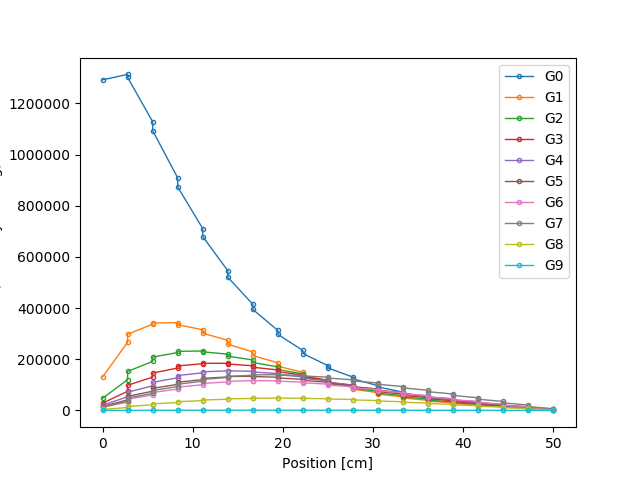
\includegraphics[width=12cm]{results/scflux_graphite_beam_1.png}
\caption{Group scalar fluxes for a high energy beam incident on a graphite block. The $y$ axis units are in $n/cm^2s$.  Upwind numerical flux used.}
\label{gb_1}
\end{figure}

The same problem was re-run this time with the average numerical flux formulation.  This resulted in figure \ref{gb_2}.

\begin{figure}[!htbp]
\centering
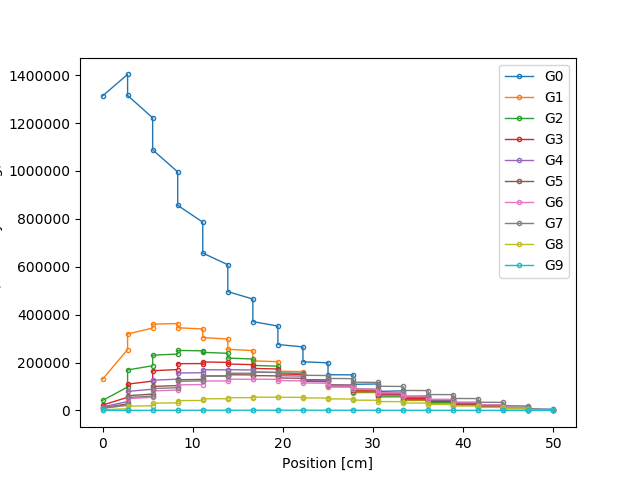
\includegraphics[width=12cm]{results/scflux_graphite_beam_2.png}
\caption{Group scalar fluxes for a high energy beam incident on a graphite block. The $y$ axis units are in $n/cm^2s$.  Average numerical flux used at element boundaries.}
\label{gb_2}
\end{figure}
Interestingly, for this problem it appears the upwind strategy provides a more accurate result. Qualitatively, the expected far-field exponential decay of the highest energy group flux is more accurately captured by the upwind flux formulation.

In the next case, a thin (0.5$[mm]$) sheet of highly absorptive pure $^{10}B$ with a density of 5$[g/cc]$ was inserted into the graphite block at 15$[cm]$.  Shown in figure \ref{gb_3}, this effectively eliminated the majority of the thermal neutron current passing through the region resulting in a sharp dip in thermal flux near the sheet, followed by thermal neutron recovery further away since there are still neutrons down scattering into the lower energy groups over the whole domain. Expectedly, the boron had little influence on the higher energy groups.  The first case was executed with 20 elements followed by a fine mesh run with 60 elements.

\begin{figure}
        \centering
        \begin{minipage}{.48\textwidth}
            \centering
            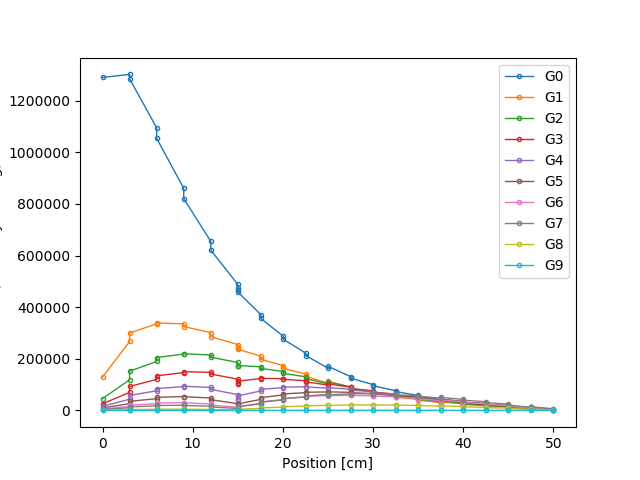
\includegraphics[width=8cm]{results/scflux_graphite_beam_3.png}
            \caption{Coarse mesh solution of the graphite block with a $^{10}B$ sheet at 15$[cm]$. }
            \label{gb_3}
        \end{minipage}%
        \begin{minipage}{.48\textwidth}
            \centering
            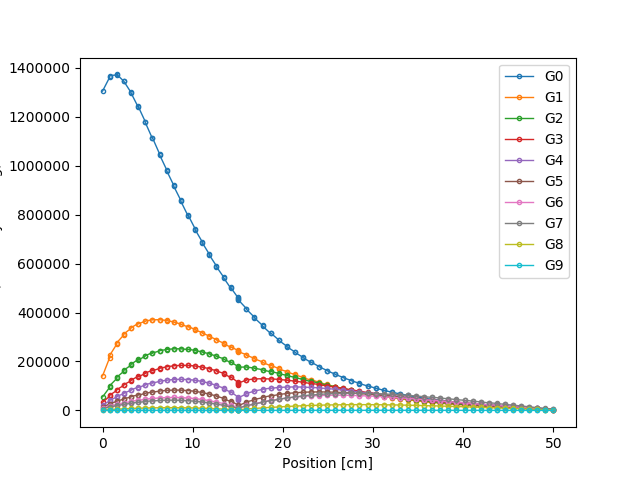
\includegraphics[width=8cm]{results/scflux_graphite_beam_4.png}
            \caption{Fine mesh solution. 
       }
        \end{minipage}
    \end{figure}